\documentclass[]{article}
\usepackage{lmodern}
\usepackage{amssymb,amsmath}
\usepackage{ifxetex,ifluatex}
\usepackage{fixltx2e} % provides \textsubscript
\ifnum 0\ifxetex 1\fi\ifluatex 1\fi=0 % if pdftex
  \usepackage[T1]{fontenc}
  \usepackage[utf8]{inputenc}
\else % if luatex or xelatex
  \ifxetex
    \usepackage{mathspec}
  \else
    \usepackage{fontspec}
  \fi
  \defaultfontfeatures{Ligatures=TeX,Scale=MatchLowercase}
\fi
% use upquote if available, for straight quotes in verbatim environments
\IfFileExists{upquote.sty}{\usepackage{upquote}}{}
% use microtype if available
\IfFileExists{microtype.sty}{%
\usepackage{microtype}
\UseMicrotypeSet[protrusion]{basicmath} % disable protrusion for tt fonts
}{}
\usepackage[margin=1in]{geometry}
\usepackage{hyperref}
\hypersetup{unicode=true,
            pdftitle={Report},
            pdfauthor={Drunken Master 2},
            pdfborder={0 0 0},
            breaklinks=true}
\urlstyle{same}  % don't use monospace font for urls
\usepackage{color}
\usepackage{fancyvrb}
\newcommand{\VerbBar}{|}
\newcommand{\VERB}{\Verb[commandchars=\\\{\}]}
\DefineVerbatimEnvironment{Highlighting}{Verbatim}{commandchars=\\\{\}}
% Add ',fontsize=\small' for more characters per line
\usepackage{framed}
\definecolor{shadecolor}{RGB}{248,248,248}
\newenvironment{Shaded}{\begin{snugshade}}{\end{snugshade}}
\newcommand{\KeywordTok}[1]{\textcolor[rgb]{0.13,0.29,0.53}{\textbf{#1}}}
\newcommand{\DataTypeTok}[1]{\textcolor[rgb]{0.13,0.29,0.53}{#1}}
\newcommand{\DecValTok}[1]{\textcolor[rgb]{0.00,0.00,0.81}{#1}}
\newcommand{\BaseNTok}[1]{\textcolor[rgb]{0.00,0.00,0.81}{#1}}
\newcommand{\FloatTok}[1]{\textcolor[rgb]{0.00,0.00,0.81}{#1}}
\newcommand{\ConstantTok}[1]{\textcolor[rgb]{0.00,0.00,0.00}{#1}}
\newcommand{\CharTok}[1]{\textcolor[rgb]{0.31,0.60,0.02}{#1}}
\newcommand{\SpecialCharTok}[1]{\textcolor[rgb]{0.00,0.00,0.00}{#1}}
\newcommand{\StringTok}[1]{\textcolor[rgb]{0.31,0.60,0.02}{#1}}
\newcommand{\VerbatimStringTok}[1]{\textcolor[rgb]{0.31,0.60,0.02}{#1}}
\newcommand{\SpecialStringTok}[1]{\textcolor[rgb]{0.31,0.60,0.02}{#1}}
\newcommand{\ImportTok}[1]{#1}
\newcommand{\CommentTok}[1]{\textcolor[rgb]{0.56,0.35,0.01}{\textit{#1}}}
\newcommand{\DocumentationTok}[1]{\textcolor[rgb]{0.56,0.35,0.01}{\textbf{\textit{#1}}}}
\newcommand{\AnnotationTok}[1]{\textcolor[rgb]{0.56,0.35,0.01}{\textbf{\textit{#1}}}}
\newcommand{\CommentVarTok}[1]{\textcolor[rgb]{0.56,0.35,0.01}{\textbf{\textit{#1}}}}
\newcommand{\OtherTok}[1]{\textcolor[rgb]{0.56,0.35,0.01}{#1}}
\newcommand{\FunctionTok}[1]{\textcolor[rgb]{0.00,0.00,0.00}{#1}}
\newcommand{\VariableTok}[1]{\textcolor[rgb]{0.00,0.00,0.00}{#1}}
\newcommand{\ControlFlowTok}[1]{\textcolor[rgb]{0.13,0.29,0.53}{\textbf{#1}}}
\newcommand{\OperatorTok}[1]{\textcolor[rgb]{0.81,0.36,0.00}{\textbf{#1}}}
\newcommand{\BuiltInTok}[1]{#1}
\newcommand{\ExtensionTok}[1]{#1}
\newcommand{\PreprocessorTok}[1]{\textcolor[rgb]{0.56,0.35,0.01}{\textit{#1}}}
\newcommand{\AttributeTok}[1]{\textcolor[rgb]{0.77,0.63,0.00}{#1}}
\newcommand{\RegionMarkerTok}[1]{#1}
\newcommand{\InformationTok}[1]{\textcolor[rgb]{0.56,0.35,0.01}{\textbf{\textit{#1}}}}
\newcommand{\WarningTok}[1]{\textcolor[rgb]{0.56,0.35,0.01}{\textbf{\textit{#1}}}}
\newcommand{\AlertTok}[1]{\textcolor[rgb]{0.94,0.16,0.16}{#1}}
\newcommand{\ErrorTok}[1]{\textcolor[rgb]{0.64,0.00,0.00}{\textbf{#1}}}
\newcommand{\NormalTok}[1]{#1}
\usepackage{longtable,booktabs}
\usepackage{graphicx,grffile}
\makeatletter
\def\maxwidth{\ifdim\Gin@nat@width>\linewidth\linewidth\else\Gin@nat@width\fi}
\def\maxheight{\ifdim\Gin@nat@height>\textheight\textheight\else\Gin@nat@height\fi}
\makeatother
% Scale images if necessary, so that they will not overflow the page
% margins by default, and it is still possible to overwrite the defaults
% using explicit options in \includegraphics[width, height, ...]{}
\setkeys{Gin}{width=\maxwidth,height=\maxheight,keepaspectratio}
\IfFileExists{parskip.sty}{%
\usepackage{parskip}
}{% else
\setlength{\parindent}{0pt}
\setlength{\parskip}{6pt plus 2pt minus 1pt}
}
\setlength{\emergencystretch}{3em}  % prevent overfull lines
\providecommand{\tightlist}{%
  \setlength{\itemsep}{0pt}\setlength{\parskip}{0pt}}
\setcounter{secnumdepth}{0}
% Redefines (sub)paragraphs to behave more like sections
\ifx\paragraph\undefined\else
\let\oldparagraph\paragraph
\renewcommand{\paragraph}[1]{\oldparagraph{#1}\mbox{}}
\fi
\ifx\subparagraph\undefined\else
\let\oldsubparagraph\subparagraph
\renewcommand{\subparagraph}[1]{\oldsubparagraph{#1}\mbox{}}
\fi

%%% Use protect on footnotes to avoid problems with footnotes in titles
\let\rmarkdownfootnote\footnote%
\def\footnote{\protect\rmarkdownfootnote}

%%% Change title format to be more compact
\usepackage{titling}

% Create subtitle command for use in maketitle
\newcommand{\subtitle}[1]{
  \posttitle{
    \begin{center}\large#1\end{center}
    }
}

\setlength{\droptitle}{-2em}

  \title{Report}
    \pretitle{\vspace{\droptitle}\centering\huge}
  \posttitle{\par}
    \author{Drunken Master 2}
    \preauthor{\centering\large\emph}
  \postauthor{\par}
      \predate{\centering\large\emph}
  \postdate{\par}
    \date{Due 5 November 2018}


\begin{document}
\maketitle

{
\setcounter{tocdepth}{3}
\tableofcontents
}
\pagebreak

\subsection{Introduction}\label{introduction}

Bootstrapping is a nonparametric approach to statistical inference that
implements Monte Carlo type simulations whereby a sampling distribution
is built by generating a large number of random samples from the
original dataset. Repeating calculations a large number of times, say
1000000 times, can become slow to compute. Therefore, the use of
efficient and fast code is essential.

This is project aimed to improve and produce two fast and efficient
bootstrap functions. The original functions to be improved were provided
by Donovan (2018). The function \emph{lmBoot} was improved using R 3.5.1
software (R, 2018), while the program \emph{SASBoot} was improved using
SAS 9.4 (SAS Institute, Cary NC) software.

A short example analysis was given for each function. The fitness
dataset from Rawlings (1998) contains measurements of the following
seven variables obtained from 31 men:

• Age: Age in years\\
• Weight: Weight in kg\\
• Oxygen: Oxygen intake rate, ml per kg body weight per minute\\
• RunTime: time to run 1.5 miles in minutes\\
• RestPulse: heart rate while resting\\
• RunPulse: heart rate at end of run\\
• MaxPulse: maximum heart rate recorded while running

A linear model was set up in each analysis and the bootstrap was used to
generate confidence intervals for each of the covariates of intervals.
Conclusions to hypothesis tests about the significance of the
relationship between the response and the parameter estimates can be
drawn using bootstrap methods depending on whether the confidence
interval contains zero, one then fails to reject the null hypothesis, or
if it does not contain zero, one can reject the null hypothesis.

\pagebreak

\subsection{R}\label{r}

\subsubsection{\texorpdfstring{\emph{The function
lmBoot}}{The function lmBoot}}\label{the-function-lmboot}

The function \emph{lmBoot} uses bootstrap sampling methods to calculate
parameter estimates for the intercept and slope parameters produced by a
linear regression.

The function takes in two arguments:

\begin{itemize}
\tightlist
\item
  inputData: the dataset that will be used for sampling, where the
  response variable is in the first column and the remainder of the
  columns contain the covariates of interest.
\item
  nBoot: The number of bootstrap samples to compute.
\end{itemize}

The function outputs:

\begin{itemize}
\tightlist
\item
  BootResults: An array with the number of rows equivalent to the nBoot
  argument and as many columns as there are Beta coeficients; i.e.~for
  the intercept and covariates.
\end{itemize}

\subsubsection{\texorpdfstring{\emph{Changes made to
lmBoot}}{Changes made to lmBoot}}\label{changes-made-to-lmboot}

\begin{enumerate}
\def\labelenumi{\arabic{enumi}.}
\tightlist
\item
  The function \emph{lmBoot\_imp} (see Appendix A.2) was the result of
  three major changes to \emph{lmBoot}.
\end{enumerate}

\begin{itemize}
\tightlist
\item
  The original \emph{lmBoot} function only produced bootstrap samples
  for one covariate while \emph{lmBoot\_imp} produces bootstrap
  estimates for a multiple number of covariates.
\item
  The use of the \emph{lm} function was removed and the beta
  coefficients were calculated using matrix calculations instead.
\end{itemize}

\[
\beta = (X^TX)^{-1}X^TY
\]

\begin{itemize}
\tightlist
\item
  \emph{forloops} are relatively slow and inefficient. Therefore, the
  \emph{forloop} was replaced using \emph{sapply} which applies a
  function to each element of a matrix. The function called
  \emph{bootLM} (see Appendix A.1) was written to carry out the
  bootstrap algorithm.
\end{itemize}

\begin{enumerate}
\def\labelenumi{\arabic{enumi}.}
\setcounter{enumi}{1}
\tightlist
\item
  The function \emph{lmBoot\_par} (see Appendix A.3) further improves
  \emph{lmBoot\_imp} using parallisation. This allows the the execution
  of the function to be split up across multiple cores rather than just
  using 1. (The results for execution times of \emph{lmBoot\_par}
  produced in this report were produced using three cores).
\end{enumerate}

Table 1 illustrates differences in runtime for three different versions
of the lmBoot function; the original, an improved version and a
parallelised version. Each function was timed on how long it took to
resample 100, 1000, 10000, 100000 and 1000000 samples.

\begin{longtable}[]{@{}llll@{}}
\caption{Changes in Runtime (in seconds) of lmBoot}\tabularnewline
\toprule
Samples & lmBoot & lmBoot Improved & lmBoot Parallised\tabularnewline
\midrule
\endfirsthead
\toprule
Samples & lmBoot & lmBoot Improved & lmBoot Parallised\tabularnewline
\midrule
\endhead
100 & 0.079 & 0.025 & 1.337\tabularnewline
1000 & 0.941 & 0.134 & 0.893\tabularnewline
10000 & 8.502 & 0.777 & 1.148\tabularnewline
1e+05 & 127.289 & 6.604 & 3.81\tabularnewline
1e+06 & - & 87.17 & 40.999\tabularnewline
\bottomrule
\end{longtable}

Original boot fucntion (lmBoot) run speed for 100,000 samples = 127.289
secs Final boot function (lmBoot\_4) run speed for 100,000 samples =
0.37 secs Overall speed increase was seen to be 126.919 secs.

Each function was also profiled for the execution of 10000 samples, the
results for which can be found in Appendix A.4.

\subsubsection{\texorpdfstring{\emph{Microbenchmark}}{Microbenchmark}}\label{microbenchmark}

Table 2 contains the results of microbenchmark comparison between the
builtin \emph{Boot} function and the final \emph{lmBoot\_par} function.
Each function was executed 10 times and the mean time taken to run the
function is shown. The microbenchmark was run for 100, 1000, 10000 and
100000 samples. For smaller numbers of samples, less than 1000 samples,
the \emph{Boot} function executes faster than the \emph{lmBoot\_par}
function. However, as the sample size increases \emph{lmBoot\_par}
performs faster than the \emph{boot} function.

\begin{longtable}[]{@{}rrr@{}}
\caption{Microbenchmark comparison (in milliseconds) between lmBoot\_par
and Boot}\tabularnewline
\toprule
Samples & lmBoot\_par & Boot\tabularnewline
\midrule
\endfirsthead
\toprule
Samples & lmBoot\_par & Boot\tabularnewline
\midrule
\endhead
1e+02 & 922.0006 & 198.1029\tabularnewline
1e+03 & 1306.5800 & 1822.5090\tabularnewline
1e+04 & 1534.3260 & 16156.0050\tabularnewline
1e+05 & 5.7670 & 151.1306\tabularnewline
\bottomrule
\end{longtable}

\subsubsection{\texorpdfstring{\emph{Example analysis using
lmBoot}}{Example analysis using lmBoot}}\label{example-analysis-using-lmboot}

An example analysis was conducted using the fitness data set. A linear
model was set up with Oxygen as the response and the remaining six
variables as the predictors. The bootstrap 95\% confidence intervals
produced by lmBoot\_par were then used to test the null hypothesis that
there is no relationship between Oxygen and each covariate, i.e.
\(\beta_i = 0\).

\begin{longtable}[]{@{}lrr@{}}
\caption{95\% Confidence Intervals for Parameter
Estimates}\tabularnewline
\toprule
& 2.5\% & 97.5\%\tabularnewline
\midrule
\endfirsthead
\toprule
& 2.5\% & 97.5\%\tabularnewline
\midrule
\endhead
Intercept & 79.660 & 121.086\tabularnewline
Age & -0.435 & -0.008\tabularnewline
Weight & -0.162 & 0.063\tabularnewline
RunTime & -3.293 & -1.843\tabularnewline
RestPulse & -0.180 & 0.098\tabularnewline
RunPulse & -0.558 & -0.084\tabularnewline
MaxPulse & -0.040 & 0.522\tabularnewline
\bottomrule
\end{longtable}

\begin{figure}
\centering
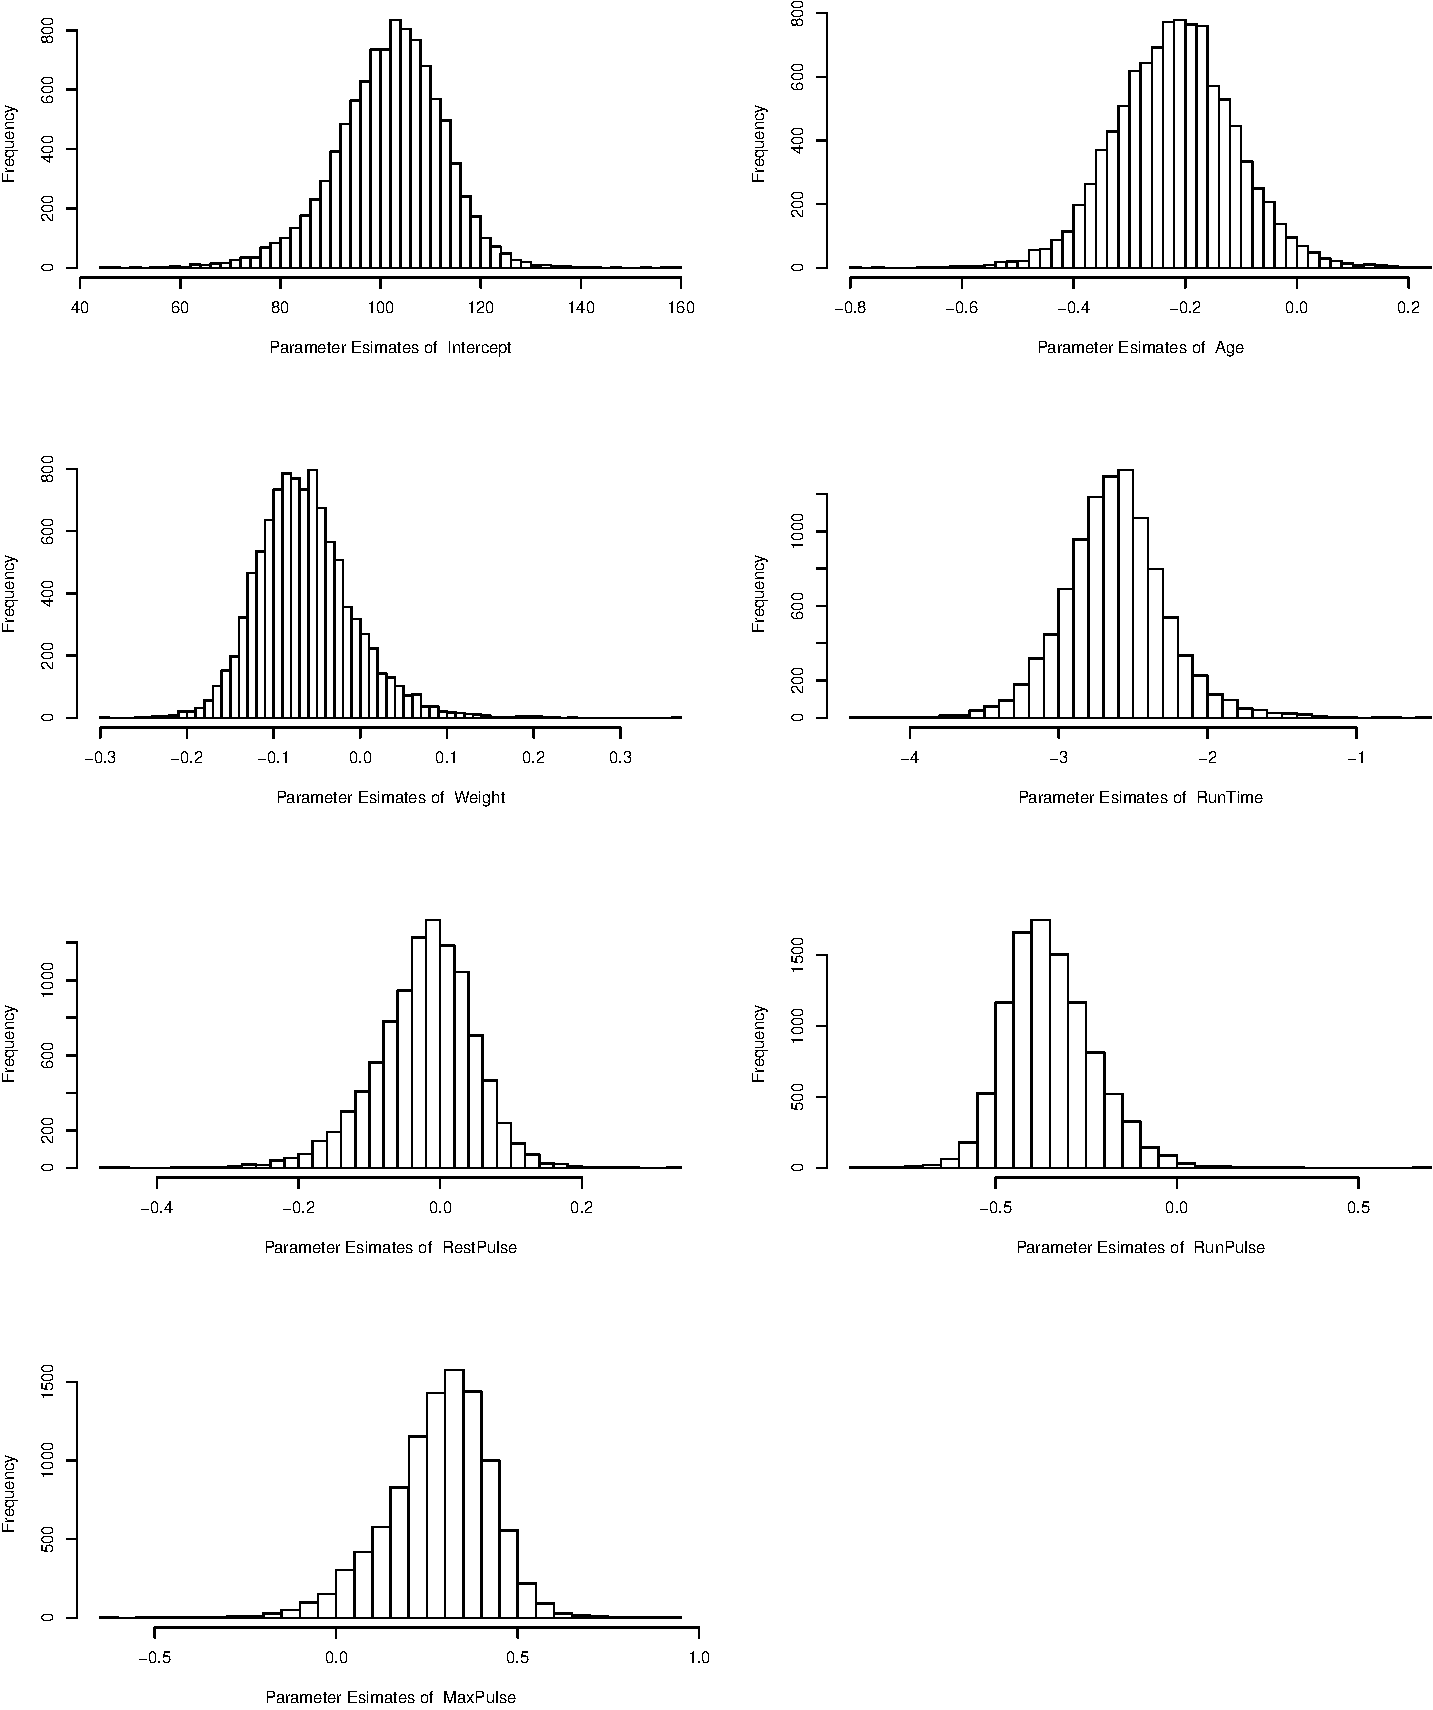
\includegraphics{Report_files/figure-latex/rcode-1.pdf}
\caption{\label{fig:rcode} Bootstrap Distributions of Parameter
Estimates}
\end{figure}

Table 3 displays the 95\% confidence intervals for the estimates of the
intercept and six covariates used in the linear regression. Figure 1
illustrates the distribution of 10000 bootstrap estimates for the same
parameters. The confidence intervals for the Age, RunTime, and RunPulse
parameter estimates do not contain zero, suggesting that there is
evidence to conclude that a significant relationship exists between
Oxygen and these covariates at the 5\% level of significance. The
confidence intervals for the Weight, RestPulse, and MaxPulse parameter
estimates do contain zero, suggesting that there is evidence to conclude
that there is not a significant relationship between Oxygen and these
covariates at the 5\% level of significance.

\pagebreak 

\subsection{SAS}\label{sas}

\subsubsection{\texorpdfstring{\emph{The program
SASBoot}}{The program SASBoot}}\label{the-program-sasboot}

The macro program \emph{SASBoot} (Appendix A.6) uses bootstrap sampling
methods to calculate estimates for the means and confidence intervals of
the slope and intercept parameters produced by a linear regression.

It takes in four agruments:

\begin{itemize}
\tightlist
\item
  NumberOfLoops: the number of bootstrap iterations.
\item
  DataSet: A SAS dataset containing the response and covariate.
\item
  XVariable: The covariate for our regression model (gen. continuous
  numeric).
\item
  YVariable: The response variable for our regression model (gen.
  continuous numeric).
\end{itemize}

The program then outputs:

\begin{itemize}
\tightlist
\item
  ResultHolder: A SAS dataset with the number of rows equivalent to the
  NumberOfLoops argument and two columns; RandomIntercept and
  RandomSlope.
\item
  output.rtf: An RTF file containing 95\% confidence intervals for the
  mean, the mean estimate for each parameter and plots of the
  distributions of the bootstrap parameters.
\end{itemize}

The function makes use of:

\begin{itemize}
\tightlist
\item
  MACRO statements to create a flexible program with input arguments.
\item
  PROC SURVEYSELECT which allows the use of random sampling to generate
  random samples from a selected or inputed dataset.
\item
  PROC REG to perform a linear regression.
\end{itemize}

\subsubsection{\texorpdfstring{\emph{Changes made to
SASBoot}}{Changes made to SASBoot}}\label{changes-made-to-sasboot}

The changes made to SASBoot were motivated, in part, by the work of
Cassel (2018) in his paper ``Don't Be Loopy: Re-Sampling and Simulation
the SAS® Way''.

\begin{enumerate}
\def\labelenumi{\arabic{enumi}.}
\tightlist
\item
  The \%do\% loop was first removed and the following code was added to
  PROC SURVEYSELECT:\\
  \emph{samprate = 1}\\
  \emph{outhits}\\
  \emph{rep = \&NumberOfLoops}
\end{enumerate}

which ensures that NumberOfLoops samples of the same size as the
original data set are produced and recorded.

\begin{enumerate}
\def\labelenumi{\arabic{enumi}.}
\setcounter{enumi}{1}
\item
  A linear regression using PROC REG was improved by introducing the
  by-variable REPLICATE. This variable is automatically produced from
  PROC SURVEYSELECT to keep track of each new bootstrap sample, and
  ensures that the linear regression is run on each sample. Thus, only
  the Result Holder Dataset was necessary, and there was no need to
  generate the Temp Dataset.
\item
  The SASFILE statement was included to upload the dataset to RAM rather
  than the hard drive before any sampling was carried out so that the
  dataset does not have to be read-in every time a resample is done.
\end{enumerate}

The program was run over increasingly large numbers of replications and
Table \#\#\# displays the runtime (in seconds) for each function. The
code used to measure the run time of the SASBoot program can be found in
Appendix A.8 (H, 2012).

\begin{longtable}[]{@{}llll@{}}
\caption{Changes in Runtime of SASBoot}\tabularnewline
\toprule
Samples & RegBoot & SASBoot & SASBoot (with rtf output)\tabularnewline
\midrule
\endfirsthead
\toprule
Samples & RegBoot & SASBoot & SASBoot (with rtf output)\tabularnewline
\midrule
\endhead
100 & 17.868 & 0.235 & 4.828\tabularnewline
1000 & 169.445 & 0.265 & 5.159\tabularnewline
10000 & 1732.052 & 0.714 & 6.535\tabularnewline
100000 & - & 5.22 & 11.381\tabularnewline
\bottomrule
\end{longtable}

\subsubsection{\texorpdfstring{\emph{Example analysis using
SASBoot}}{Example analysis using SASBoot}}\label{example-analysis-using-sasboot}

An example analysis was conducted using the fitness dataset. A linear
model was set up with Oxygen as the response and Weight as the
covariate. The bootstrap 95\% confidence intervals produced by SASBoot
were then used to test the null hypothesis that there is no significant
relationship between Oxygen and Weight, i.e. \(\beta_i = 0\).

\begin{longtable}[]{@{}lll@{}}
\caption{95\% Confidence Intervals for Parameter
Estimates}\tabularnewline
\toprule
Parameter & 2.5\% & 97.5\%\tabularnewline
\midrule
\endfirsthead
\toprule
Parameter & 2.5\% & 97.5\%\tabularnewline
\midrule
\endhead
Intercept & 36.4824 & 73.159\tabularnewline
Weight & -0.32842 & 0.13533\tabularnewline
\bottomrule
\end{longtable}

Table 5 displays the 95\% confidence intervals for the estimates of the
intercept and Weight parameters. Figure 2 and Figure 3 illustrate the
distribution of 1000 bootstrap estimates for the intercept and Weight
parameters. The confidence interval for the intercept term (36.48,
73.15) does not contain 0 which suggested that the estimator is not
signicant at the 5\% level. The confidence interval for Weight (-0.32,
0.13) did contain 0 which suggested that the estimator is signicant at
the 5\% level.

\begin{figure}
\centering
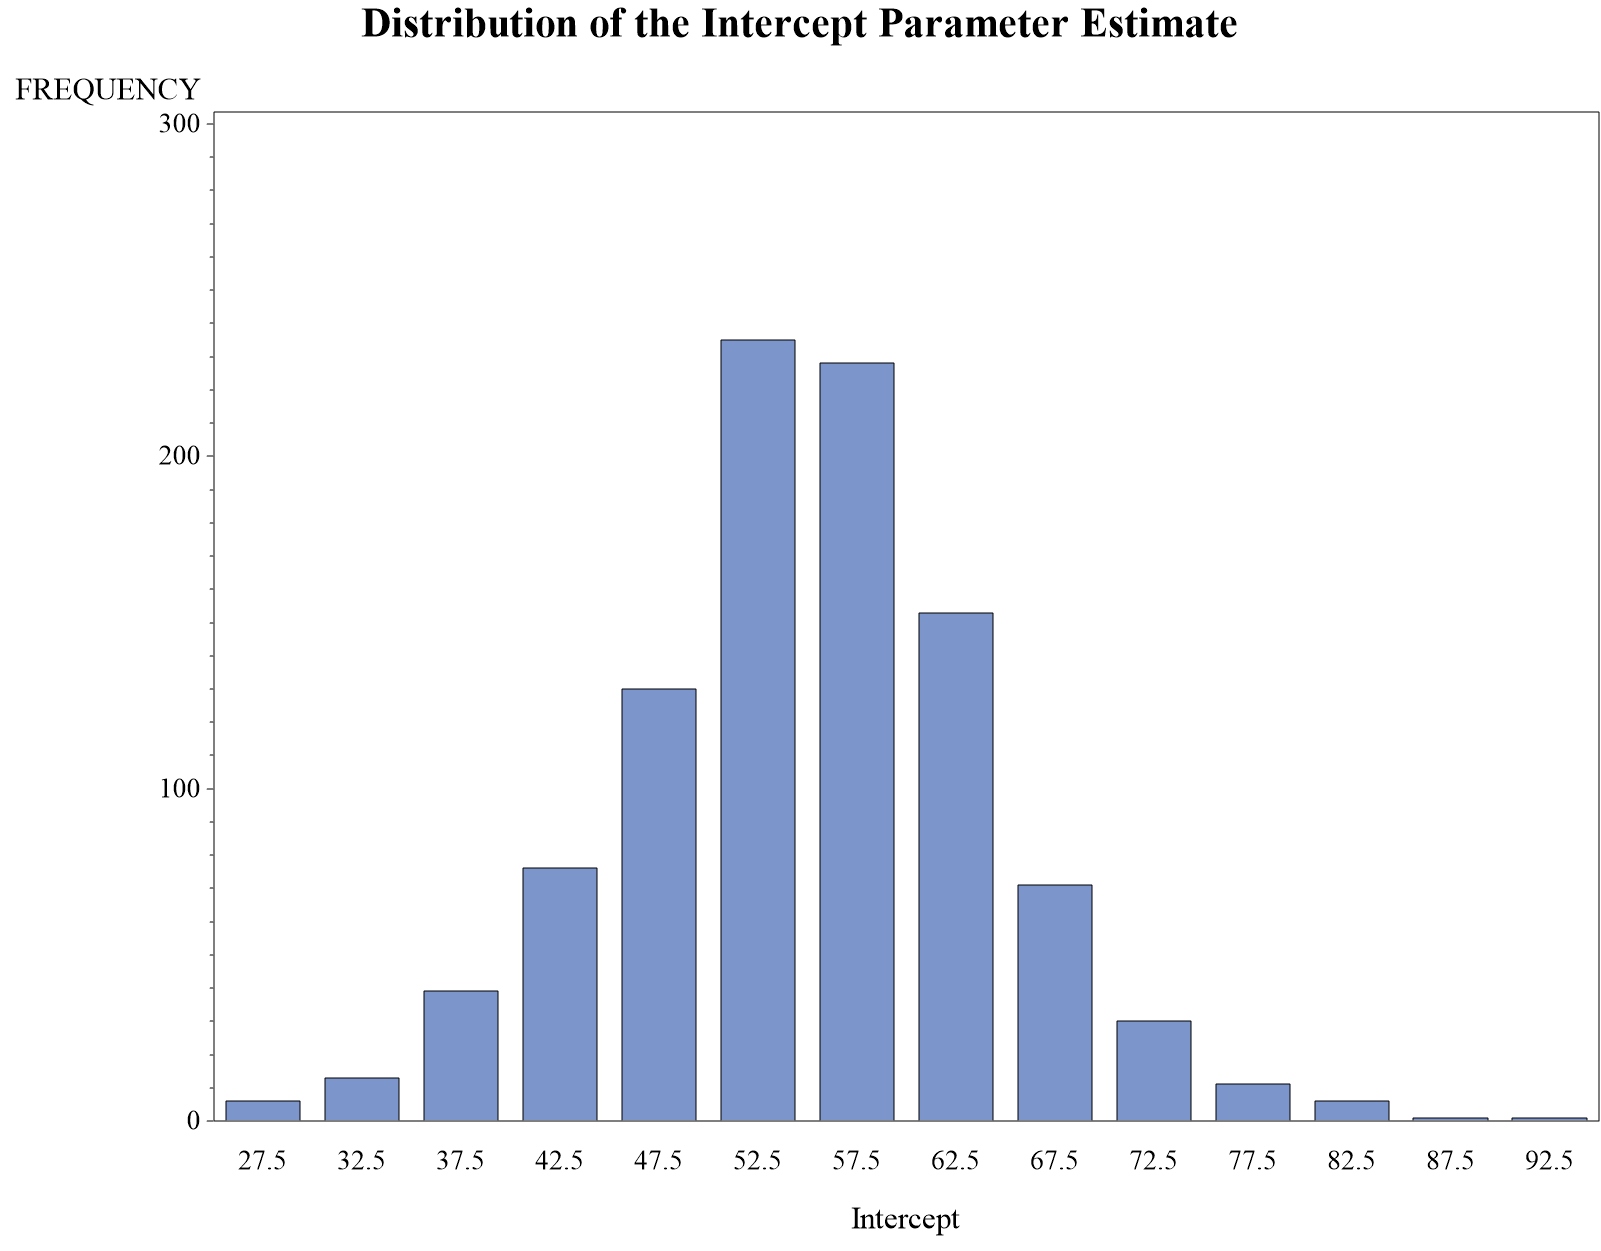
\includegraphics[width=0.75000\textwidth]{SAS Figures/SAS intercept distribution.png}
\caption{The distribution of the intercept parameter estimates}
\end{figure}

\begin{figure}
\centering
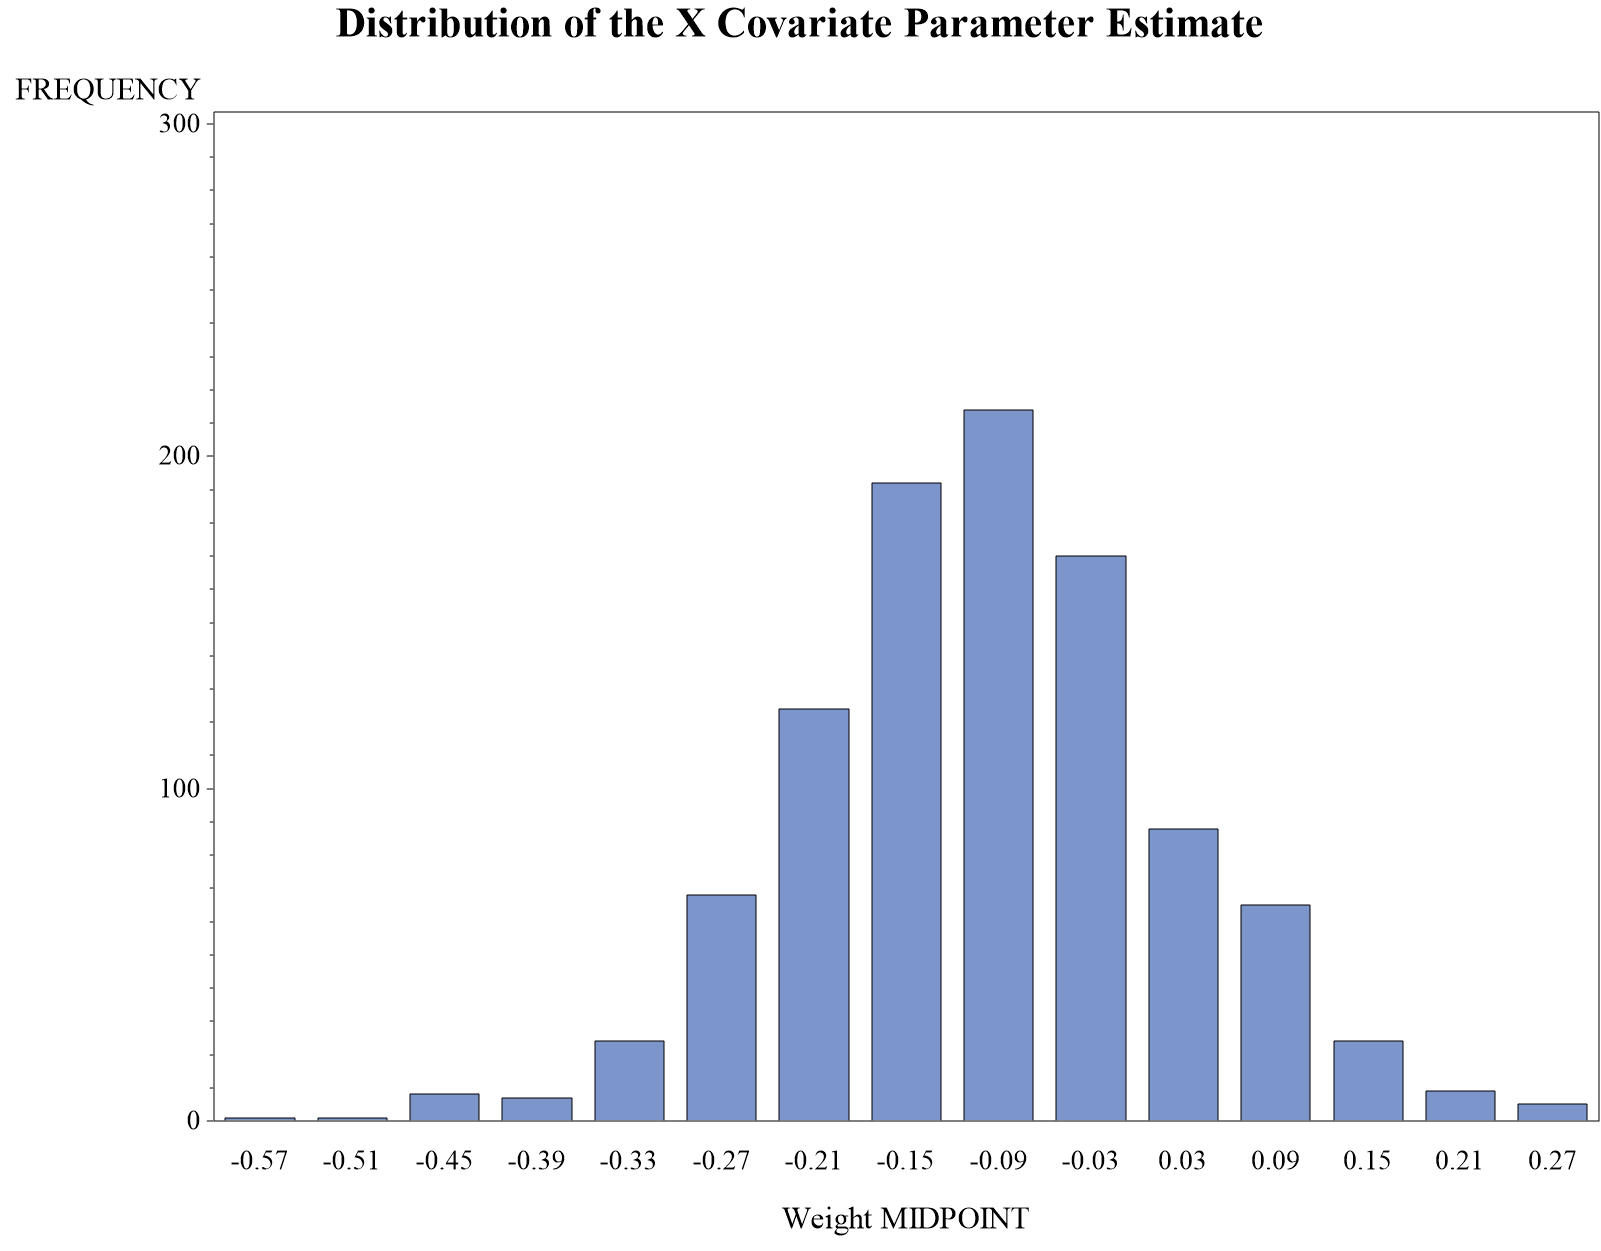
\includegraphics[width=0.75000\textwidth]{SAS Figures/SAS weight distribution.png}
\caption{The distribution of the parameter estimates for Weight}
\end{figure}

\pagebreak 

\subsection{References}\label{references}

Cassell, D. (2018). Don't Be Loopy: Re-Sampling and Simulation the SAS®
Way. {[}online{]}. Available at:
\url{http://www2.sas.com/proceedings/forum2007/183-2007.pdf} {[}Accessed
26 Oct. 2018{]}.

Donovan, C. (2018). MT5763 Project 2 - code collaboration and computer
intensive inference. {[}Online{]}.

H, J. (2012). To calculate SAS program run time. {[}online{]}. Available
at:
\url{http://sashowto.blogspot.com/2012/06/to-calculate-sas-program-run-time.html}
{[}Accessed 26 Oct. 2018{]}.

R Core Team (2018). R: A language and environment for statistical
computing. R Foundation for Statistical Computing, Vienna, Austria.
Available at: \url{https://www.R-project.org/}.

SAS 9.4, SAS Institute Inc., Cary, NC, USA.

\pagebreak 

\subsection{Appendix}\label{appendix}

\subsubsection{A.1 The Bootlm Function}\label{a.1-the-bootlm-function}

\begin{Shaded}
\begin{Highlighting}[]
\NormalTok{bootLM <-}\StringTok{ }\ControlFlowTok{function}\NormalTok{(samples, inputData, index)\{}
  \CommentTok{#Purpose: Generate the linear regression beta coefficients}
  \CommentTok{#Inputs: samples: a dataframe containing the indices for the bootstrap samples}
  \CommentTok{#        inputData: a dataframe containing the response variable, which must be }
  \CommentTok{#        in the first column of the dataframe, and the covariates of interest}
  \CommentTok{#        index: the index of the position in the BootResults that Bootlm }
  \CommentTok{#        should be applied to}
  \CommentTok{#Outputs: Beta: An matrix containing the parameter estimates from a linear }
  \CommentTok{#         regression}
  
\NormalTok{  bootData <-}\StringTok{ }\NormalTok{inputData[samples[, index], ]}
\NormalTok{  Xmat <-}\StringTok{ }\NormalTok{bootData[, }\OperatorTok{-}\DecValTok{1}\NormalTok{]}
\NormalTok{  Ymat <-}\StringTok{ }\NormalTok{bootData[, }\DecValTok{1}\NormalTok{]}
\NormalTok{  beta <-}\StringTok{ }\KeywordTok{solve}\NormalTok{(}\KeywordTok{t}\NormalTok{(Xmat)}\OperatorTok\NormalTok{Xmat)}\OperatorTok\KeywordTok{t}\NormalTok{(Xmat)}\OperatorTok\NormalTok{Ymat}
  \KeywordTok{return}\NormalTok{(beta)}
\NormalTok{\}}
\end{Highlighting}
\end{Shaded}

\subsubsection{A.2 The lmBoot\_imp
Function}\label{a.2-the-lmboot_imp-function}

\begin{Shaded}
\begin{Highlighting}[]
\NormalTok{lmBoot_imp <-}\StringTok{ }\ControlFlowTok{function}\NormalTok{(inputData, nBoot)\{}
  \CommentTok{#Purpose: Generate a large number of linear regression beta coefficients using}
  \CommentTok{#         bootstrap methods.}
  \CommentTok{#Inputs: inputData: a dataframe containing the response variable, which must be }
  \CommentTok{#        in the first column of the dataframe, and the covariates of interest}
  \CommentTok{#        nBoot: the number of bootstrap samples to generate.}
  \CommentTok{#Outputs: BootResults: An arraycontaing the parameter estimates of each }
  \CommentTok{#         each bootstrap sample.}
  \CommentTok{#         ConfidenceIntervals: A matrix containing 95% confidence intervals }
  \CommentTok{#         for each parameter.}
  
  \CommentTok{#Calculate the number of observations in the dataset }
\NormalTok{  nObs <-}\StringTok{ }\KeywordTok{nrow}\NormalTok{(inputData)}
  
  \CommentTok{#Create a sample dataset with a column of 1s for the intercept}
\NormalTok{  sampleData <-}\StringTok{ }\KeywordTok{as.matrix}\NormalTok{(}\KeywordTok{cbind}\NormalTok{(inputData[, }\DecValTok{1}\NormalTok{], }\DecValTok{1}\NormalTok{, inputData[, }\OperatorTok{-}\DecValTok{1}\NormalTok{]))}
  
  \CommentTok{# Create the a matrix of indices for the bootstrap samples}
\NormalTok{  bootSamples <-}\StringTok{ }\KeywordTok{matrix}\NormalTok{(}\KeywordTok{sample}\NormalTok{(}\DecValTok{1}\OperatorTok{:}\KeywordTok{nrow}\NormalTok{(inputData), nObs }\OperatorTok{*}\StringTok{ }\NormalTok{nBoot, }\DataTypeTok{replace =}\NormalTok{ T), }
                        \DataTypeTok{nrow =}\NormalTok{ nObs, }\DataTypeTok{ncol =}\NormalTok{ nBoot)}
  
  \CommentTok{#Create an empty array to store results}
\NormalTok{  bootResults <-}\StringTok{ }\KeywordTok{array}\NormalTok{(}\DataTypeTok{dim =} \KeywordTok{c}\NormalTok{(nBoot, }\KeywordTok{ncol}\NormalTok{(sampleData[, }\OperatorTok{-}\DecValTok{1}\NormalTok{]))) }

  \CommentTok{#Use sapply to apply bootLM to bootResults matrix}
\NormalTok{  bootResults <-}\StringTok{ }\KeywordTok{sapply}\NormalTok{(}\DecValTok{1}\OperatorTok{:}\NormalTok{nBoot, bootLM, }\DataTypeTok{inputData =}\NormalTok{ sampleData, }
                        \DataTypeTok{samples =}\NormalTok{ bootSamples)}
\NormalTok{  bootResults <-}\StringTok{ }\KeywordTok{t}\NormalTok{(}\KeywordTok{as.matrix}\NormalTok{(bootResults))}
  
  \KeywordTok{return}\NormalTok{(bootResults)}
\NormalTok{\}}
\end{Highlighting}
\end{Shaded}

\subsubsection{A.3 The lmBoot\_par
Function}\label{a.3-the-lmboot_par-function}

\begin{Shaded}
\begin{Highlighting}[]
\KeywordTok{library}\NormalTok{(doParallel)}

\NormalTok{lmBoot_par <-}\StringTok{ }\ControlFlowTok{function}\NormalTok{(inputData, nBoot)\{}
  \CommentTok{#Purpose: Generate a large number of linear regression beta coefficients using}
  \CommentTok{#         bootstrap methods.}
  \CommentTok{#Inputs: inputData: a dataframe containing the response variable, which must be }
  \CommentTok{#        in the first column of the dataframe, and the covariates of interest}
  \CommentTok{#        nBoot: the number of bootstrap samples to generate.}
  \CommentTok{#Outputs: BootResults: An arraycontaing the parameter estimates of each }
  \CommentTok{#         each bootstrap sample.}
  \CommentTok{#         ConfidenceIntervals: A matrix containing 95% confidence intervals }
  \CommentTok{#         for each parameter.}
  
  \CommentTok{#Calculate the number of observations in the dataset }
\NormalTok{  nObs <-}\StringTok{ }\KeywordTok{nrow}\NormalTok{(inputData)}
  
  \CommentTok{#Create the sample data with 1s for the intercept}
\NormalTok{  sampleData <-}\StringTok{ }\KeywordTok{as.matrix}\NormalTok{(}\KeywordTok{cbind}\NormalTok{(inputData[, }\DecValTok{1}\NormalTok{], }\DecValTok{1}\NormalTok{, inputData[, }\OperatorTok{-}\DecValTok{1}\NormalTok{]))}
  
  \CommentTok{#Set up parallisation}
\NormalTok{  nCores <-}\StringTok{ }\KeywordTok{detectCores}\NormalTok{()}
\NormalTok{  myClust <-}\StringTok{ }\KeywordTok{makeCluster}\NormalTok{(nCores }\OperatorTok{-}\StringTok{ }\DecValTok{1}\NormalTok{, }\DataTypeTok{type =} \StringTok{"PSOCK"}\NormalTok{)}
  \KeywordTok{registerDoParallel}\NormalTok{(myClust)}
  
  \CommentTok{# Create the samples}
\NormalTok{  bootSamples <-}\StringTok{ }\KeywordTok{matrix}\NormalTok{(}\KeywordTok{sample}\NormalTok{(}\DecValTok{1}\OperatorTok{:}\KeywordTok{nrow}\NormalTok{(inputData), nObs }\OperatorTok{*}\StringTok{ }\NormalTok{nBoot, }\DataTypeTok{replace =}\NormalTok{ T), }
                        \DataTypeTok{nrow =}\NormalTok{ nObs, }\DataTypeTok{ncol =}\NormalTok{ nBoot)}
  
  \CommentTok{#Use parallised sapply to apply bootLM to bootResults matrix}
\NormalTok{  bootResults <-}\StringTok{ }\KeywordTok{matrix}\NormalTok{(}\OtherTok{NA}\NormalTok{, nBoot, }\KeywordTok{ncol}\NormalTok{(sampleData[, }\OperatorTok{-}\DecValTok{1}\NormalTok{]))}
\NormalTok{  bootResults <-}\StringTok{ }\KeywordTok{parSapply}\NormalTok{(myClust, }\DecValTok{1}\OperatorTok{:}\NormalTok{nBoot, bootLM, }\DataTypeTok{inputData =}\NormalTok{ sampleData, }
                           \DataTypeTok{samples =}\NormalTok{ bootSamples)}

  \CommentTok{#Close parallisation}
  \KeywordTok{stopCluster}\NormalTok{(myClust)}
  
  \KeywordTok{return}\NormalTok{(}\KeywordTok{t}\NormalTok{(bootResults))}
\NormalTok{\}}
\end{Highlighting}
\end{Shaded}

\pagebreak

\subsubsection{\texorpdfstring{A.4 R Profiles for \emph{lmBoot},
\emph{lmBoot\_imp} and
\emph{lmBoot\_par}}{A.4 R Profiles for lmBoot, lmBoot\_imp and lmBoot\_par}}\label{a.4-r-profiles-for-lmboot-lmboot_imp-and-lmboot_par}

\begin{figure}
\centering
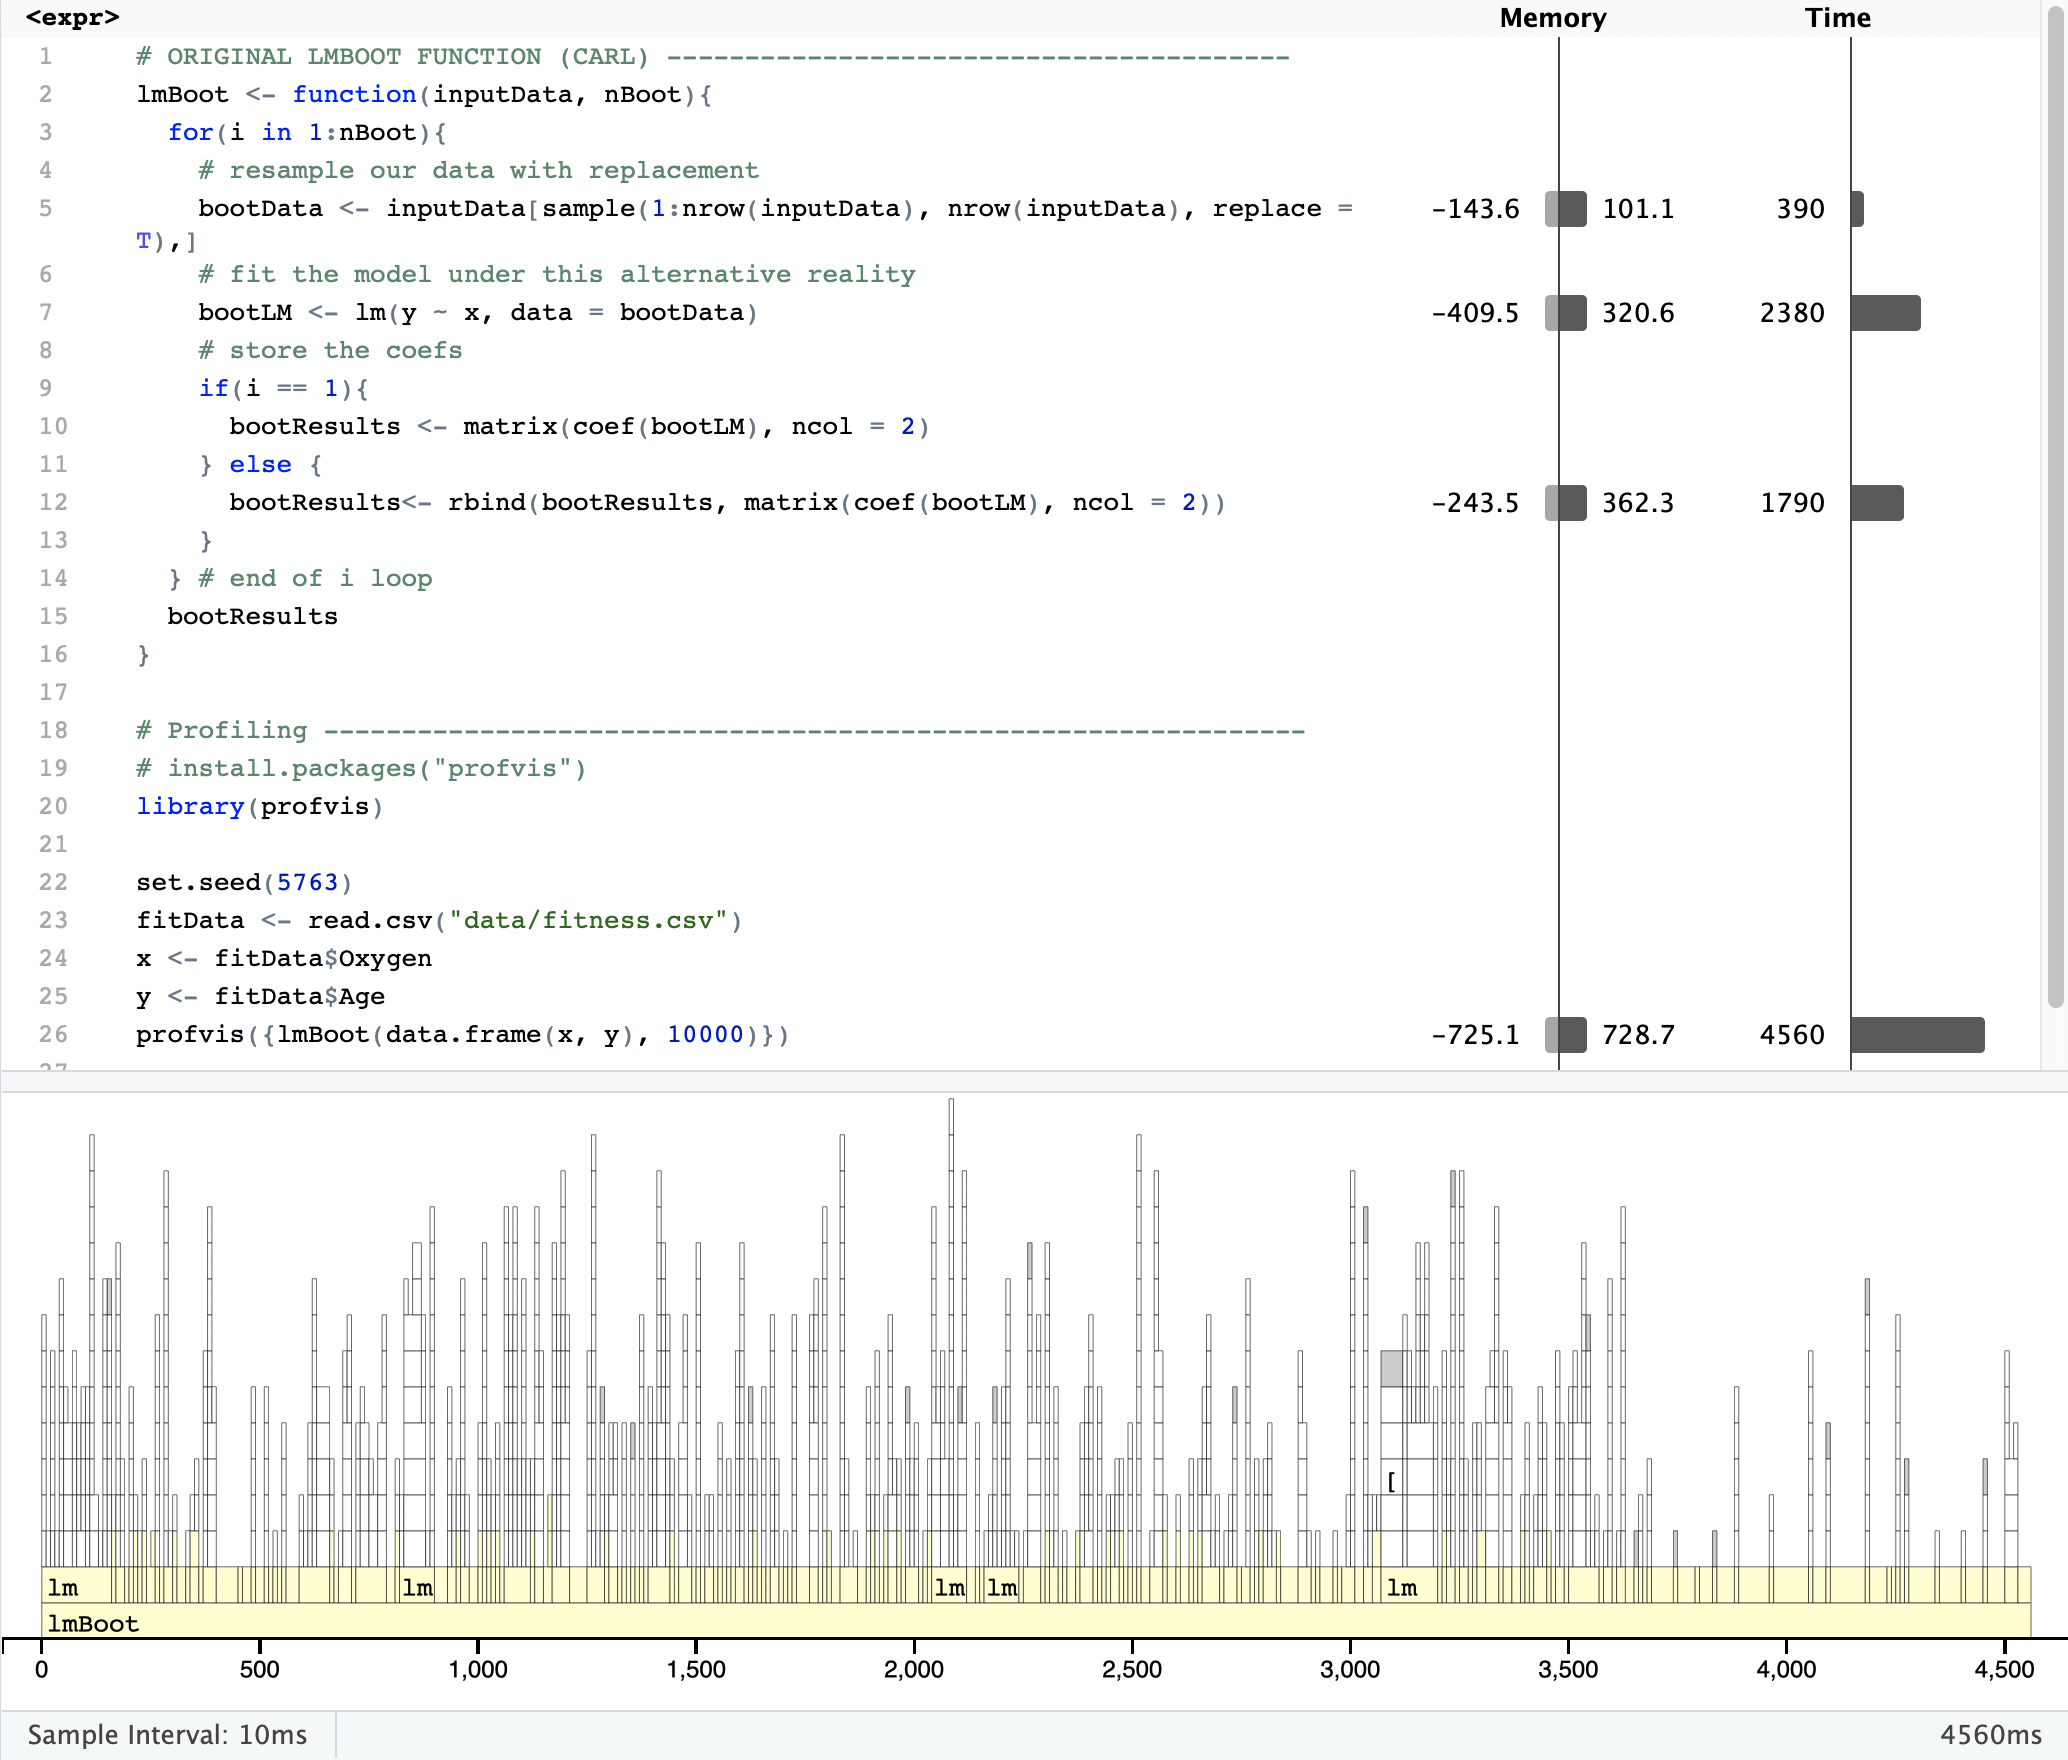
\includegraphics[width=0.69000\textwidth]{Profiling/lmBoot Profile Image.png}
\caption{R Profile for \emph{lmBoot}}
\end{figure}

\begin{figure}
\centering
\includegraphics[width=0.69000\textwidth]{Profiling/lmBoot_imp Profile Image.png}
\caption{R Profile for \emph{lmBoot\_imp}}
\end{figure}

\begin{figure}
\centering
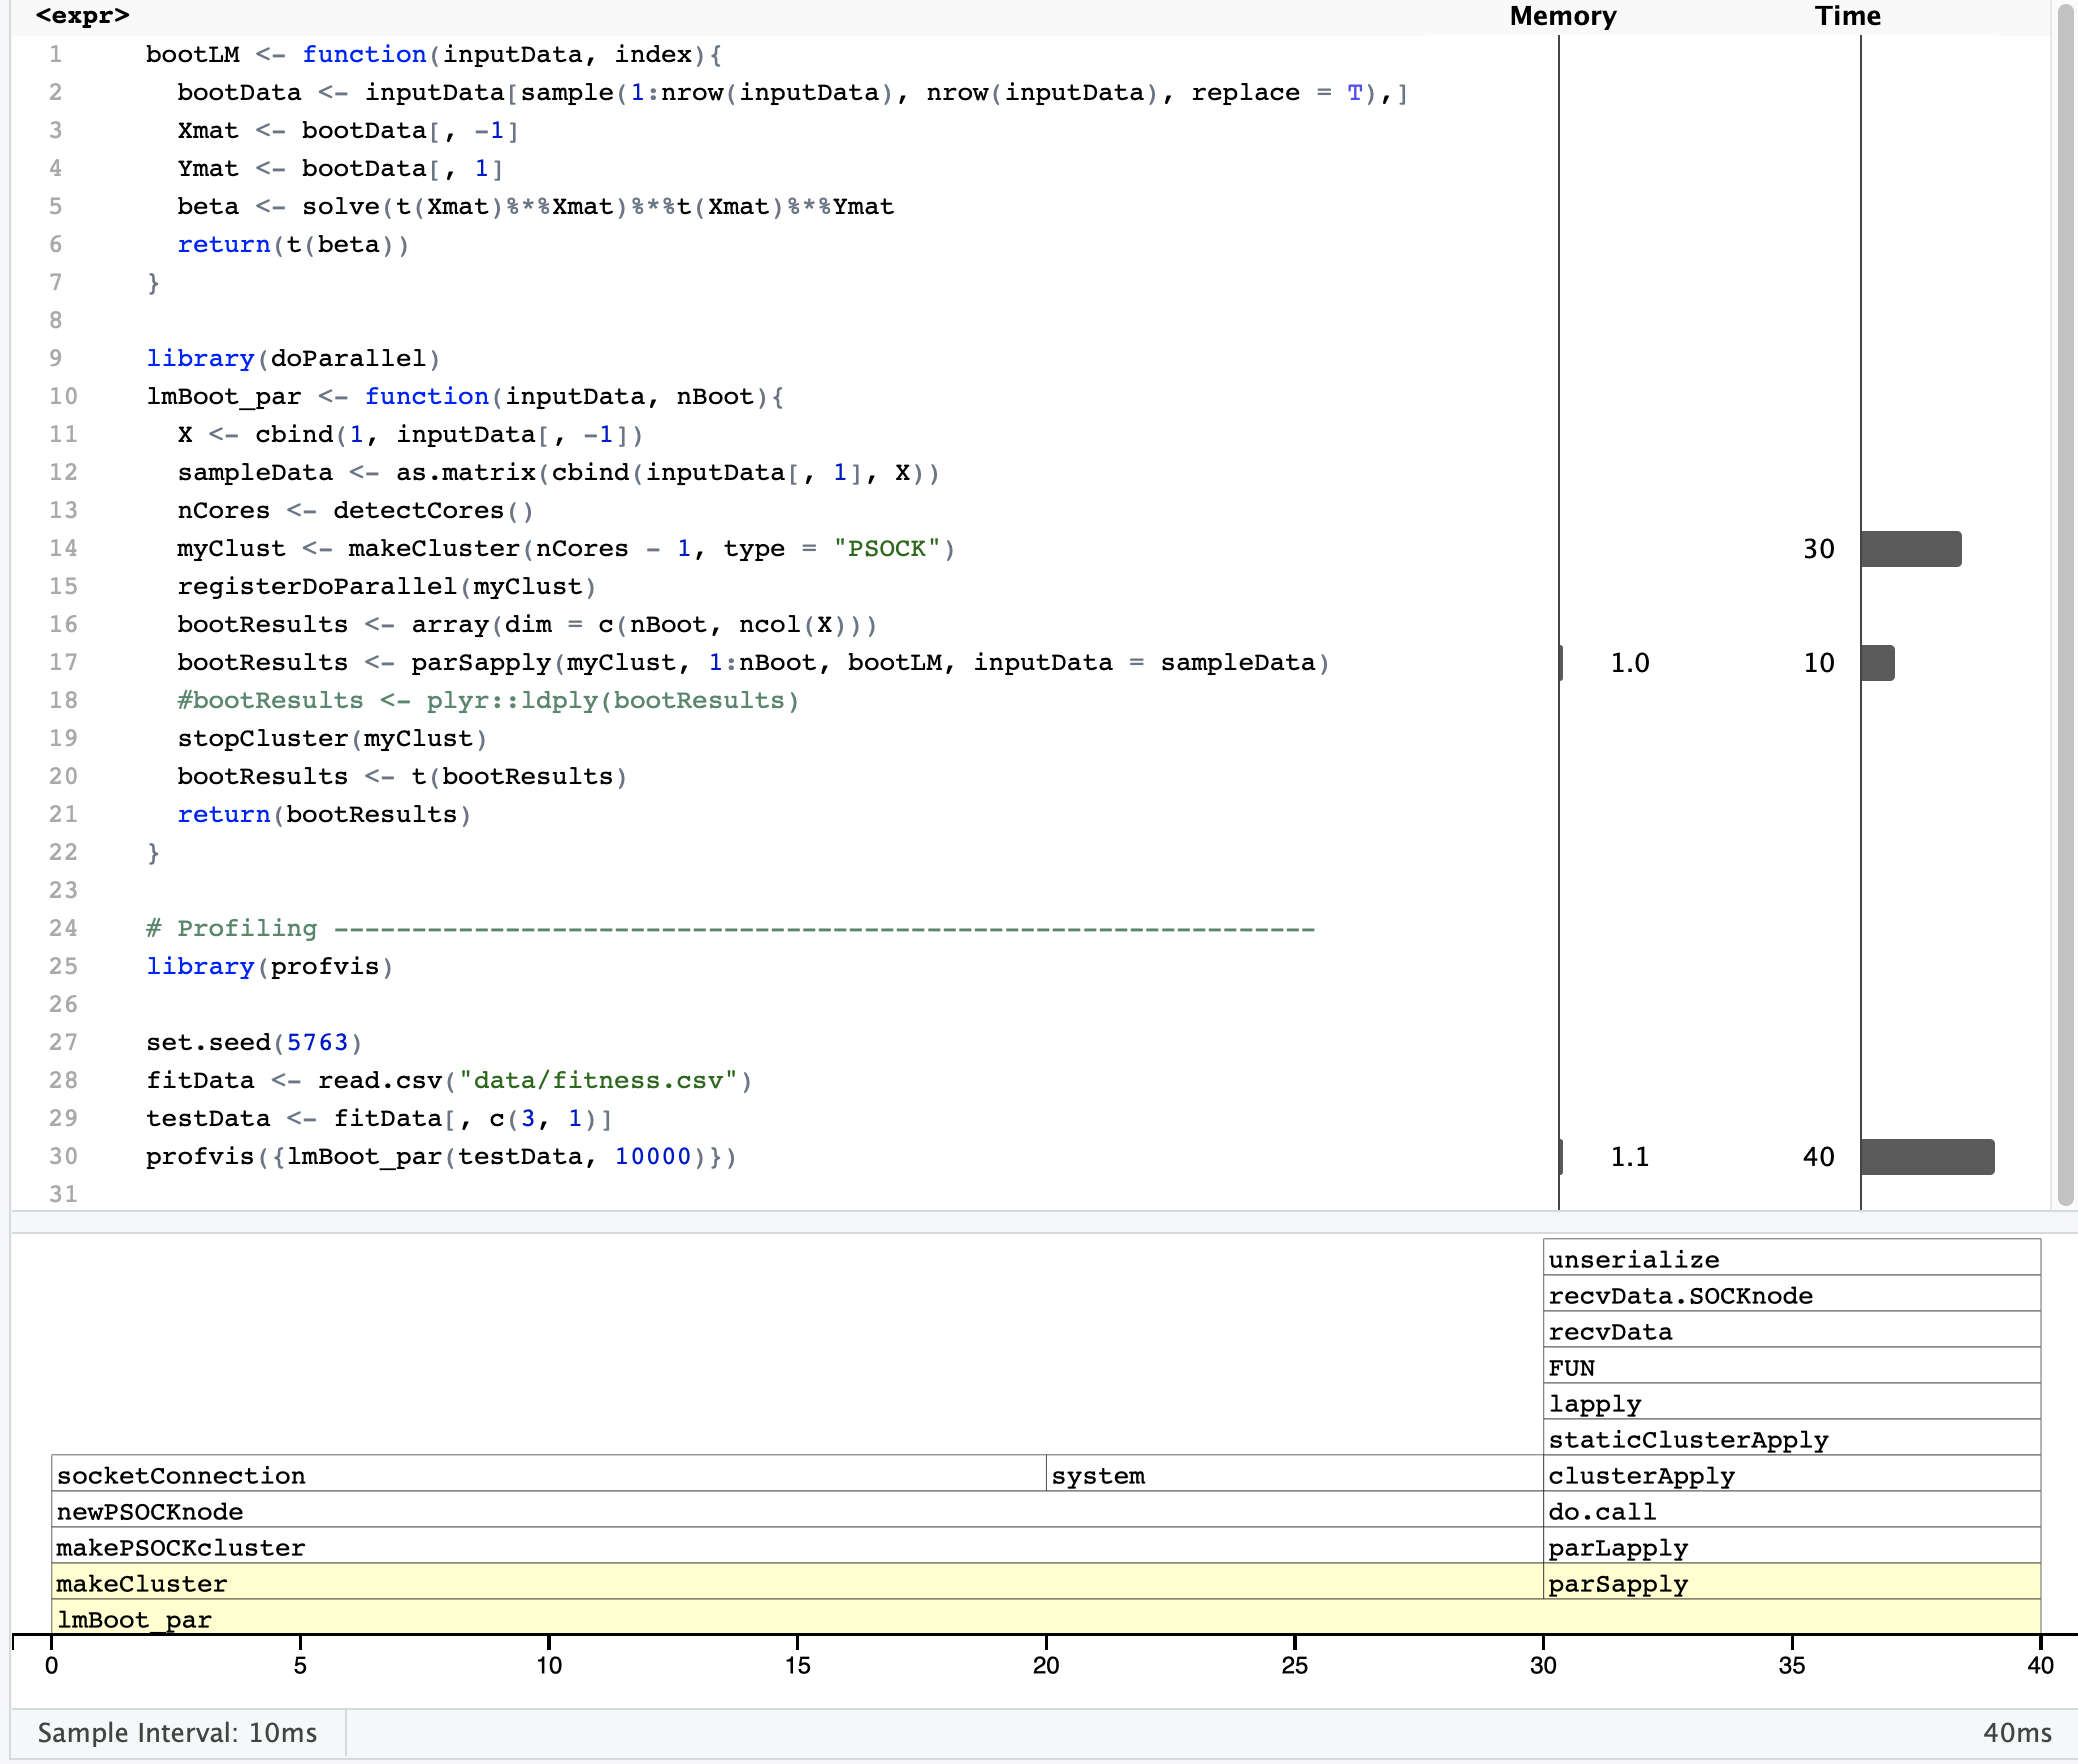
\includegraphics[width=0.69000\textwidth]{Profiling/lmBoot_par Profile Image.png}
\caption{R Profile for \emph{lmBoot\_par}}
\end{figure}

\pagebreak

\subsubsection{A.5 Bootstrap Example Analysis with
R}\label{a.5-bootstrap-example-analysis-with-r}

\begin{Shaded}
\begin{Highlighting}[]
\KeywordTok{library}\NormalTok{(dplyr)}

\NormalTok{fitData <-}\StringTok{ }\KeywordTok{read.csv}\NormalTok{(}\StringTok{"data/fitness.csv"}\NormalTok{)}
\NormalTok{testData <-}\StringTok{ }\NormalTok{fitData }\OperatorTok\StringTok{ }\KeywordTok{select}\NormalTok{(Oxygen, }\KeywordTok{everything}\NormalTok{())}
\KeywordTok{set.seed}\NormalTok{(}\DecValTok{5763}\NormalTok{)}
\NormalTok{testResults <-}\StringTok{ }\KeywordTok{lmBoot_par}\NormalTok{(testData, }\DecValTok{10000}\NormalTok{)}

\CommentTok{#Plot the distributions for each parameter}
\KeywordTok{par}\NormalTok{(}\DataTypeTok{mfrow =} \KeywordTok{c}\NormalTok{(}\DecValTok{4}\NormalTok{,}\DecValTok{2}\NormalTok{))}
\ControlFlowTok{for}\NormalTok{(i }\ControlFlowTok{in} \DecValTok{1}\OperatorTok{:}\KeywordTok{ncol}\NormalTok{(testResults))\{}
  \KeywordTok{hist}\NormalTok{(testResults[, i], }\DataTypeTok{breaks =} \DecValTok{50}\NormalTok{, }
       \DataTypeTok{main =} \StringTok{""}\NormalTok{, }\DataTypeTok{xlab =} \KeywordTok{paste}\NormalTok{(}\StringTok{"Parameter Esimates of "}\NormalTok{, }\KeywordTok{names}\NormalTok{(testResults[i])))}
\NormalTok{\}}
  
\CommentTok{#Confidence intervals}
\NormalTok{ciMatrix <-}\StringTok{ }\KeywordTok{matrix}\NormalTok{(}\OtherTok{NA}\NormalTok{, }\DataTypeTok{nrow =} \KeywordTok{ncol}\NormalTok{(testResults), }\DataTypeTok{ncol =} \DecValTok{2}\NormalTok{)}
\ControlFlowTok{for}\NormalTok{(i }\ControlFlowTok{in} \DecValTok{1}\OperatorTok{:}\KeywordTok{ncol}\NormalTok{(testResults))\{}
\NormalTok{  ciMatrix[i, ] <-}\StringTok{ }\KeywordTok{quantile}\NormalTok{(testResults[,i], }\DataTypeTok{probs =} \KeywordTok{c}\NormalTok{(}\FloatTok{0.025}\NormalTok{, }\FloatTok{0.975}\NormalTok{))}
\NormalTok{\}}
\KeywordTok{colnames}\NormalTok{(ciMatrix) <-}\StringTok{ }\KeywordTok{c}\NormalTok{(}\StringTok{"2.5%"}\NormalTok{, }\StringTok{"97.5%"}\NormalTok{)}
\KeywordTok{rownames}\NormalTok{(ciMatrix) <-}\StringTok{ }\KeywordTok{c}\NormalTok{(}\StringTok{"Intercept"}\NormalTok{, }\KeywordTok{names}\NormalTok{(testData[}\OperatorTok{-}\DecValTok{1}\NormalTok{]))}
\end{Highlighting}
\end{Shaded}

\subsubsection{A.6 The SASBoot Program}\label{a.6-the-sasboot-program}

\begin{Shaded}
\begin{Highlighting}[]
\NormalTok{%macro }\KeywordTok{SASBoot}\NormalTok{(NumberOfLoops, DataSet, XVariable, YVariable);}

\OperatorTok{/}\ErrorTok{*}\StringTok{ }\NormalTok{Load data set to RAM and generate random samples of the data }\OperatorTok{*}\ErrorTok{/}
\ErrorTok{/*}\StringTok{       }\NormalTok{sasfile }\OperatorTok{&}\NormalTok{DataSet load;}\OperatorTok{*}\ErrorTok{/}
\StringTok{       }\NormalTok{proc surveyselect data=}\ErrorTok{&}\NormalTok{DataSet out=BootData seed=}\OperatorTok{-}\DecValTok{23434}\NormalTok{ noprint}
\NormalTok{       method=urs samprate=}\DecValTok{1}\NormalTok{ outhits rep=}\ErrorTok{&}\NormalTok{NumberOfLoops;}
\NormalTok{       run;}
\OperatorTok{/}\ErrorTok{*}\StringTok{       }\NormalTok{sasfile }\OperatorTok{&}\NormalTok{DataSet close;}\OperatorTok{*}\ErrorTok{/}

\ErrorTok{/*}\NormalTok{Calculate and store the parameter estimates}\OperatorTok{*}\ErrorTok{/}

\StringTok{       }\NormalTok{proc reg data=BootData outest=}\KeywordTok{ParameterEstimates}\NormalTok{(}\DataTypeTok{drop=}\NormalTok{_}\OperatorTok{:}\NormalTok{) noprint;}
\NormalTok{       model }\OperatorTok{&}\NormalTok{YVariable=}\ErrorTok{&}\NormalTok{XVariable;}
\NormalTok{       by replicate;}
\NormalTok{       run;}

\OperatorTok{/}\ErrorTok{*}\NormalTok{Extract and store the columns }\ControlFlowTok{for}\NormalTok{ the intercept and X covariate}\OperatorTok{*}\ErrorTok{/}

\StringTok{       }\NormalTok{data ResultHolder;}
\NormalTok{       set ParameterEstimates;}
\NormalTok{       keep Intercept }\OperatorTok{&}\NormalTok{XVariable;}
\NormalTok{       run;}

\OperatorTok{/}\ErrorTok{*}\NormalTok{Calculate the means of the X covariate of every bootstrap sample}\OperatorTok{*}\ErrorTok{/}

\StringTok{       }\NormalTok{proc univariate data=BootData noprint;}
\NormalTok{       var }\OperatorTok{&}\NormalTok{XVariable;}
\NormalTok{       by replicate;}
\NormalTok{       output out=uniOut mean=mean}\OperatorTok{&}\NormalTok{XVariable;}
\NormalTok{       run;}

\OperatorTok{/}\ErrorTok{*}\NormalTok{Calculate }\DecValTok{95}\NormalTok{% confidence intervals }\ControlFlowTok{for}\NormalTok{ the mean of the intercept parameter estimates}\OperatorTok{*}\ErrorTok{/}

\StringTok{       }\NormalTok{proc univariate data=ResultHolder;}
\NormalTok{       var Intercept;}
\NormalTok{       output out=InterceptCI pctlpts=}\FloatTok{2.5}\NormalTok{, }\FloatTok{97.5}\NormalTok{ pctlpre=CI; }
\NormalTok{       run;}

\OperatorTok{/}\ErrorTok{*}\NormalTok{Calculate }\DecValTok{95}\NormalTok{% confidence intervals }\ControlFlowTok{for}\NormalTok{ the mean of X covariate parameter estimates}\OperatorTok{*}\ErrorTok{/}

\StringTok{       }\NormalTok{proc univariate data=ResultHolder;}
\NormalTok{       var }\OperatorTok{&}\NormalTok{XVariable;}
\NormalTok{       output out=XvarCI pctlpts=}\FloatTok{2.5}\NormalTok{, }\FloatTok{97.5}\NormalTok{ pctlpre=CI; }
\NormalTok{       run;}

       \OperatorTok{/}\ErrorTok{*}\NormalTok{Create output RTF file}\OperatorTok{*}\ErrorTok{/}

\StringTok{       }\NormalTok{ods rtf file=}\StringTok{"output.rtf"}\NormalTok{ bodytitle startpage =}\StringTok{ }\NormalTok{never;}
\NormalTok{        title1 }\StringTok{"Drunken Master 2"}\NormalTok{;}
\NormalTok{        title2 }\StringTok{"Results of SAS Bootstrap Program"}\NormalTok{;}

\NormalTok{        title4 }\StringTok{"95% Confidence Interval for the Intercept Parameter Estimate"}\NormalTok{;}

        \OperatorTok{/}\ErrorTok{*}\NormalTok{Results }\ControlFlowTok{for}\NormalTok{ the intercept parameter estimate}\OperatorTok{*}\ErrorTok{/}

\StringTok{        }\NormalTok{proc print data=InterceptCI;}
\NormalTok{        run;}
\NormalTok{        title }\StringTok{"Distribution of the Intercept Parameter Estimate"}\NormalTok{;}
\NormalTok{        proc gchart data=ResultHolder;}
\NormalTok{        vbar Intercept;}
\NormalTok{        run;}

        \OperatorTok{/}\ErrorTok{*}\NormalTok{Results }\ControlFlowTok{for}\NormalTok{ the X covariate parameter estimate}\OperatorTok{*}\ErrorTok{/}

\StringTok{        }\NormalTok{ods startpage =}\StringTok{ }\NormalTok{now;}
\NormalTok{        title }\StringTok{"95% Confidence Interval for the X Covariate Parameter Estimate"}\NormalTok{;}
\NormalTok{        proc print data=XvarCI;}
\NormalTok{        run;}

\NormalTok{        title }\StringTok{"Distribution of the X Covariate Parameter Estimate"}\NormalTok{;}
\NormalTok{        proc gchart data=ResultHolder;}
\NormalTok{        vbar }\OperatorTok{&}\NormalTok{XVariable;}
\NormalTok{        run;}

\NormalTok{        ods rtf close;}

\NormalTok{%MEND SASBoot; }\OperatorTok{/}\ErrorTok{*}\NormalTok{End of SASBoot macro}\OperatorTok{*}\ErrorTok{/}
\end{Highlighting}
\end{Shaded}

\subsubsection{A.7 Bootstrap Example Analysis with
SAS}\label{a.7-bootstrap-example-analysis-with-sas}

\begin{Shaded}
\begin{Highlighting}[]
\OperatorTok{/}\ErrorTok{*}\NormalTok{Importing the fitness data set}\OperatorTok{*}\ErrorTok{/}

\NormalTok{proc import out =}\StringTok{ }\NormalTok{Asmt2.fitness }
\NormalTok{   datafile =}\StringTok{ "C:\textbackslash{}Users}\CharTok{\textbackslash{}b}\StringTok{af3\textbackslash{}Desktop}\CharTok{\textbackslash{}f}\StringTok{itness.csv"} 
\NormalTok{   dbms =}\StringTok{ }\NormalTok{CSV REPLACE;}
\NormalTok{   getnames =}\StringTok{ }\NormalTok{YES;}
\NormalTok{   datarow =}\StringTok{ }\DecValTok{2}\NormalTok{; }
\NormalTok{run;}

\NormalTok{%}\KeywordTok{SASBoot}\NormalTok{(}\DataTypeTok{NumberOfLoops=}\DecValTok{1000}\NormalTok{, }\DataTypeTok{DataSet=}\NormalTok{Asmt2.fitness, }\DataTypeTok{XVariable=}\NormalTok{Weight, }\DataTypeTok{YVariable=}\NormalTok{Oxygen);}
\end{Highlighting}
\end{Shaded}

\subsubsection{A.8 Code to measure program runtime in
SAS}\label{a.8-code-to-measure-program-runtime-in-sas}

\begin{Shaded}
\begin{Highlighting}[]
\OperatorTok\KeywordTok{sysfunc}\NormalTok{(}\KeywordTok{datetime}\NormalTok{());}

\NormalTok{  Program of interest to be timed}

\OperatorTok\KeywordTok{sysfunc}\NormalTok{(}\KeywordTok{datetime}\NormalTok{());  }
\OperatorTok\KeywordTok{sysfunc}\NormalTok{(}\KeywordTok{putn}\NormalTok{(}\OperatorTok{&}\NormalTok{_edtm }\OperatorTok{-}\StringTok{ }\ErrorTok{&}\NormalTok{_sdtm, }\FloatTok{12.4}\NormalTok{));  }
\NormalTok{%put It took }\OperatorTok{&}\NormalTok{_runtm seconds to run the program;}
\end{Highlighting}
\end{Shaded}


\end{document}
